\section{Preliminary Performance}

\subsection{Electron response}

\begin{figure}[hbt]
\centering
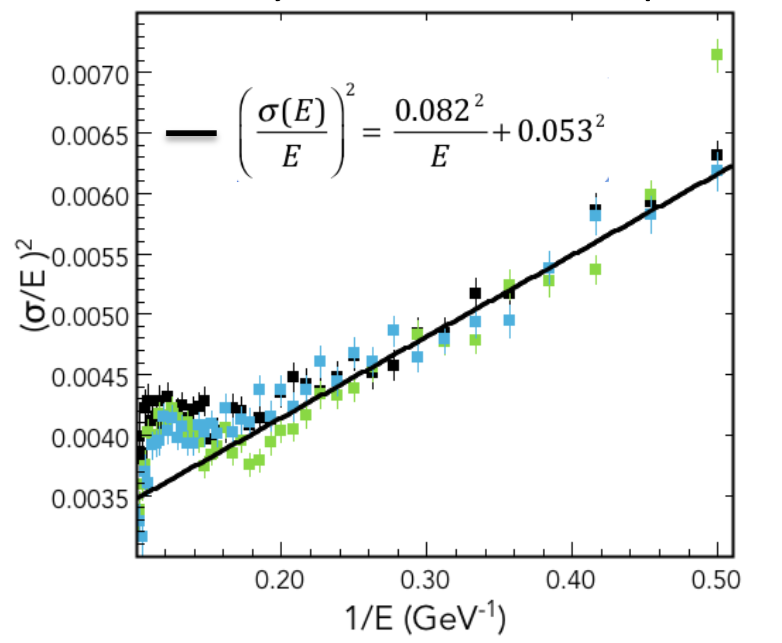
\includegraphics[width=1.0\columnwidth,keepaspectratio]{img/S10_1_3.png}
\caption[]{}
\label{fig:S10_1_2}
\end{figure}

\subsection{Position resolution}
\subsection{Reconstruction of $\pi^0\rightarrow 2\gamma$ decays}
\subsection{Neutron detection}
Clusters in the FEC not associated with any reconstructed track in the forward (DC) tracking system are designated neutrals by the event builder service.  Association of neutral PCAL clusters with ECIN and ECOU clusters are based on proximity to straight line trajectories from the CLAS12 origin.  Photons and neutrons are distinguished on the basis of the timing response, with neutrons defined as $\beta < 0.9$.  Experiments which require the exclusive measurement of neutrons in the FEC therefore require both good timing resolution and sufficient detection efficiency. 

Neutron detection in the FEC was measured by tagging neutrons using the $p\,(\,e,e'\,\pi^+\,)\,n$ reaction. Events with missing momentum pointing into the fiducial region of the FEC were selected.  True neutron hits were identified by requiring the direction of the missing momentum to be the same as the direction of a measured neutral cluster within the expected angular resolution, assuming the target center
as origin (Fig.~\ref{fig:S10_4_1}).  

\begin{figure}[hbt]
\centering
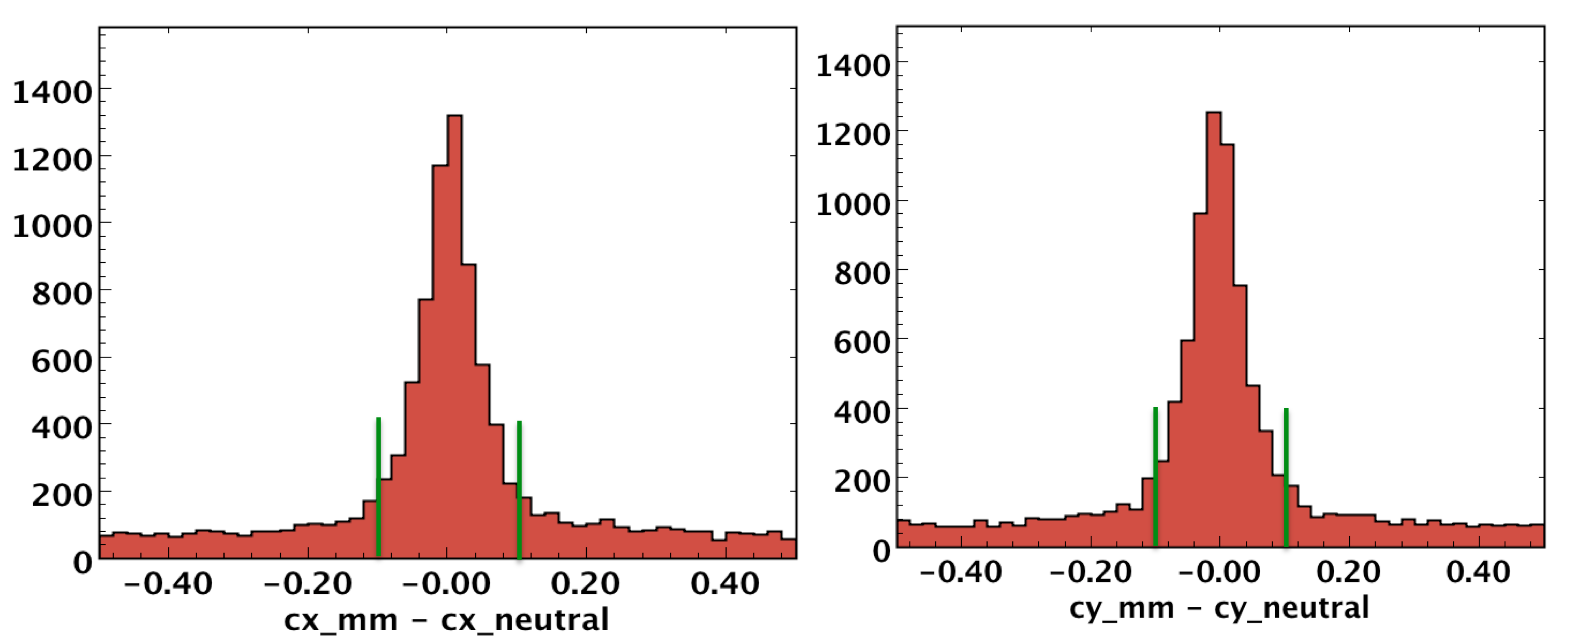
\includegraphics[width=1.0\columnwidth,keepaspectratio]{img/S10_4_1.png}
\caption[]{Differences in $\theta$ and $\phi$ between the detected neutral cluster in the FEC and the missing momentum of the tagged neutron.  The vertical lines indicate cuts used to minimize backgrounds from uncorrelated photons.}
\label{fig:S10_4_1}
\end{figure}

\begin{figure}[hbt]
\centering
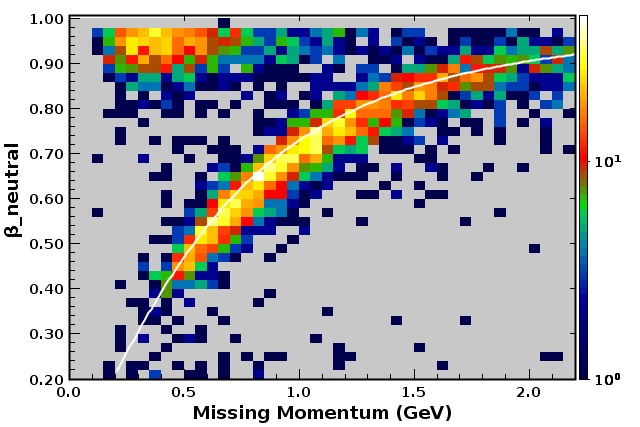
\includegraphics[width=1.0\columnwidth,keepaspectratio]{img/S10_4_2.png}
\caption[]{Correlation between the measured velocity $\beta$ calculated from neutral clusters in the FEC and the missing momentum of the tagged neutron, subject to the $\Delta\theta,\Delta\phi$ cuts shown in Figure 13.  The white line shows the expected correlation from neutrons.}
\label{fig:S10_4_2}
\end{figure}






